\documentclass[10pt,a4paper]{article}
\usepackage[a4paper,bindingoffset=0.2in,%
            left=1in,right=1in,top=1in,bottom=1in,%
            footskip=.25in]{geometry}

\usepackage[utf8x]{inputenc}
\usepackage[spanish]{babel}

\usepackage{mathtools}
\usepackage{amsmath}
\usepackage{amsfonts}
\usepackage{amssymb}

\usepackage{xcolor}
\usepackage{listingsutf8}
\usepackage{booktabs}
\usepackage{hyperref}
\usepackage{multirow}

\usepackage{caption}
\usepackage{subcaption}

\usepackage{algorithm}
\usepackage[noend]{algpseudocode}

\usepackage{graphicx}
\usepackage{tikz}
\usepackage{relsize}
\usepackage{epstopdf}

\DeclarePairedDelimiter{\ceil}{\lceil}{\rceil}

% set the default code style
\lstset{
    frame=tb, % draw a frame at the top and bottom of the code block
    tabsize=4, % tab space width
    showstringspaces=false, % don't mark spaces in strings
    numbers=left, % display line numbers on the left
    commentstyle=\color{green}, % comment color
    keywordstyle=\color{blue}, % keyword color
    stringstyle=\color{red} % string color
}

% mathy stuff
\newtheorem{theorem}{Theorem}[section]
\newtheorem{lemma}[theorem]{Lemma}
\newtheorem{proposition}[theorem]{Proposición}
\newtheorem{corollary}[theorem]{Corollary}

\newenvironment{proof}[1][Demostración]{\begin{trivlist}
\item[\hskip \labelsep {\bfseries #1}]}{\end{trivlist}}
\newenvironment{definition}[1][Definición]{\begin{trivlist}
\item[\hskip \labelsep {\bfseries #1}]}{\end{trivlist}}
\newenvironment{example}[1][Example]{\begin{trivlist}
\item[\hskip \labelsep {\bfseries #1}]}{\end{trivlist}}
\newenvironment{remark}[1][Remark]{\begin{trivlist}
\item[\hskip \labelsep {\bfseries #1}]}{\end{trivlist}}

\newcommand{\qed}{\nobreak \ifvmode \relax \else
      \ifdim\lastskip<1.5em \hskip-\lastskip
      \hskip1.5em plus0em minus0.5em \fi \nobreak
      \vrule height0.75em width0.5em depth0.25em\fi}

\title{Aprendizaje Automatico \\ Trabajo Práctico 2 \\ Un jugador inteligente del Cuatro En Línea }

%\newcommand{\order}[1]{$\mathcal{O}(#1)$}

\begin{document}

%% cover page

\maketitle

\bigskip

\begin{table}[h]
\centering
\begin{tabular}{|l l l l|}
\hline
Integrante       & \multicolumn{1}{c}{LU}     & Correo electrónico              & Carrera \\ \hline
Martin Baigorria & \multicolumn{1}{c}{575/14} & martinbaigorria@gmail.com & Computación (licenciatura) \\
Damián Furman & \multicolumn{1}{c}{936/11}& damian.a.furman@gmail.com & Computación (licenciatura)\\
Germán Abrevaya & \multicolumn{1}{c}{-} & germanabrevaya@gmail.com & Física (doctorado)\\ \hline
\end{tabular}
\end{table}

\vfill

\begin{center}
\textbf{Reservado para la cátedra}
\end{center}
\begin{table}[h]
\centering
\begin{tabular}{|l|l|l|}
\hline
Instancia       & Docente & Nota \\ \hline
Primera entrega &         &      \\ \hline
Segunda entrega &         &      \\ \hline
\end{tabular}
\end{table}

\newpage
\tableofcontents
\newpage

% end cover page

\section{Introducción}

El objetivo de este trabajo es el desarrollo de un jugador artificial `inteligente' del juego ``Cuatro en Línea". Utilizamos para esto la técnica de \textit{Q Learning} mediante la cual se representan todos los tableros posibles como distintos cuadrantes de un espacio sobre el cual es posible desplazarse hacia otros estados válidos que representan un movimiento en el tablero actual. Cada movimiento obtiene una recompensa que se plasma en el cuadrante en el cual ese movimiento se ejecutó y que se propaga hacia cuadrantes vecinos. De esta manera, el jugador progresivamente aprende cómo llegar hacia situaciones conocidas donde sabe cómo ganar, así como también, a alejarse de situaciones conocidas donde sabe que puede perder.

\section{Implementación}

\section{Experimentación}

\subsection{Q Learning Vs Random Player}

Una vez implementado nuestro jugador, decidimos testearlo haciéndolo jugar contra un jugador que elige movidas \textit{random} de entre aquellas movidas disponibles. De esta manera podemos observar si el jugador se comporta efectivamente de manera inteligente y si mejora a partir de su experiencia. Elegimos para nuestro jugador inteligente un porcentaje de jugadas aleatorias (epsilon) del 20\%, un \textit{learning rate} de 0.8 y un \textit{discount factor} de 0.9. En las figuras 1 a 3 podemos observar los resultados para treinta mil, cien mil y quinientas mil partidas jugadas entre estos dos jugadores. Se puede observar un patrón común en el que el jugador \textit{Q Learning} (curva azul) va progresivamente distanciándose respecto a la tasa de aciertos del jugador \textit{random} (curva verde).  Si bien existe una pequeña diferencia casi desde los primeros juegos, se ve una curva de forma asintótica que tiene un \textit{sweet spot} (punto de inflexión en la concavidad de la curva) al rededor de las cincuenta mil partidas jugadas, a partir del cual la tasa para cada jugador comienza a converger en valores aproximados de 0.15 y 0.82 respectivamente para el jugador \textit{random} y \textit{Q Learning}
\\

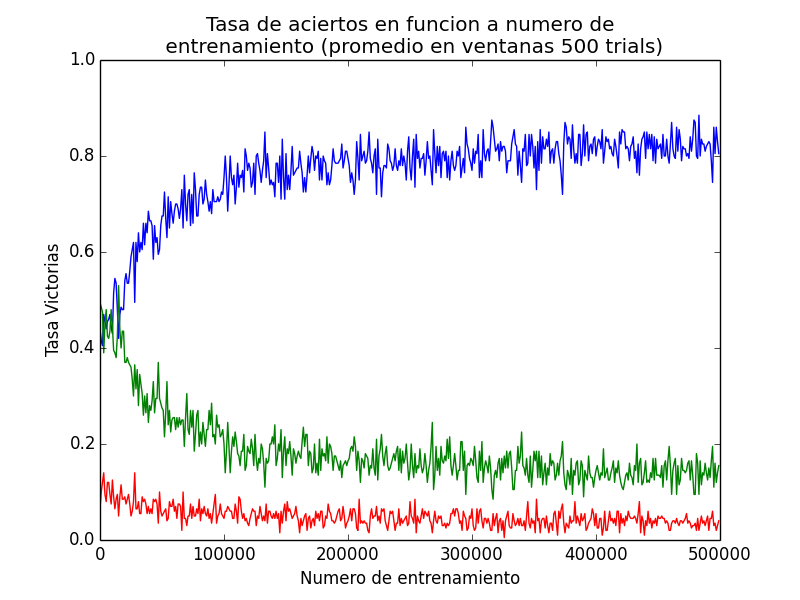
\includegraphics[scale=0.25]{q_vs_random_500_with_ties.png}
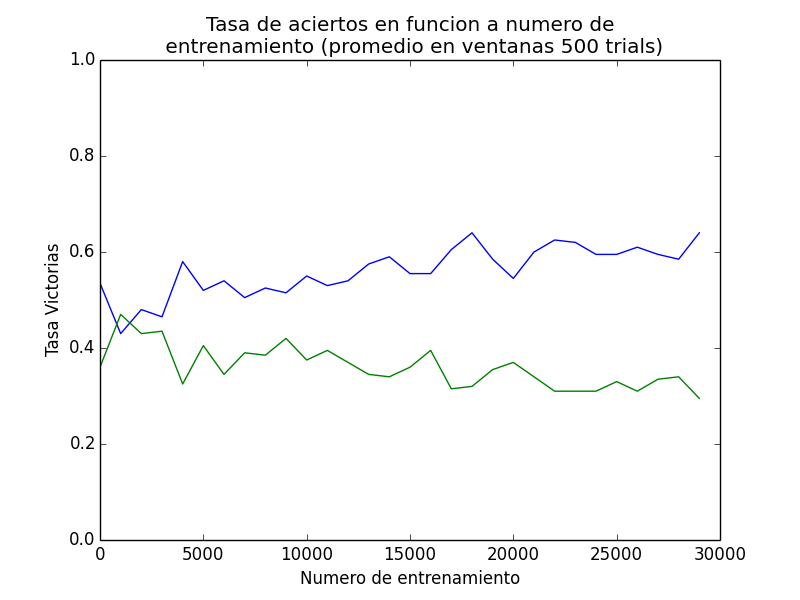
\includegraphics[scale=0.25]{random_vs_qlearning_30000.png}
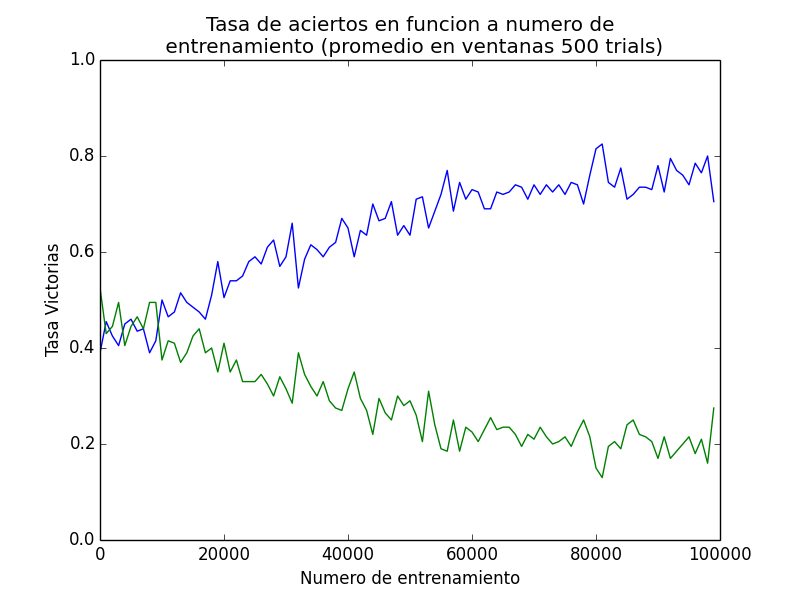
\includegraphics[scale=0.25]{random_vs_qlearning_100000.png}


A su vez, junto con el resultado correspondiente a las quinientas mil partidas jugadas, incluimos también la tasa promedio de partidas empatadas (curva roja). Según nuestra hipótesis, la cantidad de partidas empatadas debería tender a disminuir en la medida que nuestro jugador inteligente `mejora', lo que puede observarse en el gráfico donde los empates presentan un comportamiento decreciente a medida que aumenta la cantidad de entrenamientos, que comienza en valores cercanos a 0.1 y termina en valores cercanos a 0.05.
\\

\subsection{Q Learning vs Q Learning}

Luego de experimentar con un jugador random, decidimos experimentar con dos jugadores entrenados de la misma manera, con iguales hiperparámetros, que partiesen de las mismas condiciones. Ambos jugadores tienen la misma probabilidad de arrancar jugando. Queremos observar así cómo se comporta nuestro algoritmo de aprendizaje ante otro jugador que también mejora con el paso del tiempo. Partimos de la hipótesis de que luego de un período en el cual alguno de los jugadores podría sacarle cierta ventaja al otro, deberían tender a estabilizarse en la medida en que completen su entrenamiento debido a que éste se realiza, para ambos, en las mismas condiciones. A su vez, esperabamos que el \textit{ratio} de los empates aumentase en la medida que ambos jugadores mejoraran ya que el que Q learner además de aprender a ganar aprende a evitar perder.

\begin{center}
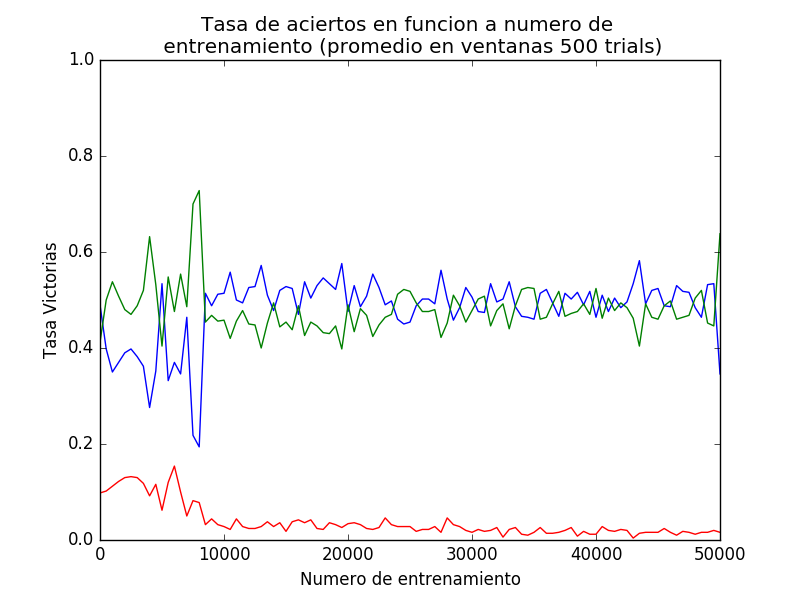
\includegraphics[scale=0.5]{QlearnervsQlearner50000.png}
\end{center}

Lo que terminamos observando iba en contra de nuestra intuicion La cantidad de empates que observabamos para diferentes combinaciones de hiperparametros era muy grande y comenzamos a sospechar que algo no estaba bien. Sin embargo, luego conjeturamos que en realidad el jugador que arranca el juego siempre tiene una estrategia ganadora. Para testear esta hipotesis, cambiamos la forma en que se entrenaban los jugadores para que sistematicamente uno siempre arrancara primero.

\begin{center}
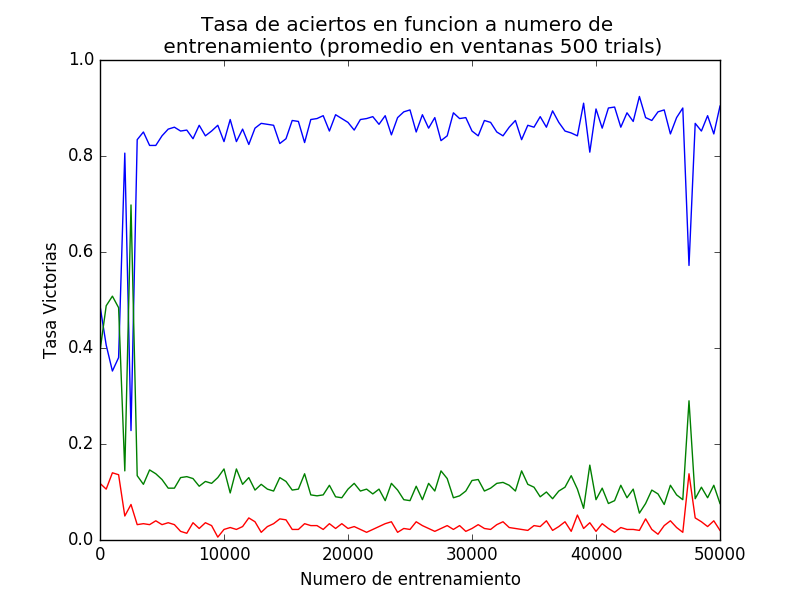
\includegraphics[scale=0.5]{qvsq_arranca.png}
\end{center}

Finalmente se confirmo nuestra hipotesis. Efectivamente el jugador que arranca siempre tiene ventaja. Conjeturamos que debe existir una estrategia ganadora para el jugador que arranca en 4 en Linea para tableros simetricos de dimension $n \geq 5$. La prueba formal excede el scope de este trabajo (y por lo que vemos ya esta estudiado).

\subsection{Variaciones sobre Épsilon}

El hiperparametro epsilon determina la probabilidad de que un jugador decida hacer una jugada aleatoria, en vez de seguir la estrategia 'optima' dada por el valor de su funcion Q. Este hiperparametro en primera instancia le permite al jugador explorar el espacio de jugadas. En primera instancia explorar es deseable. Sin embargo, a medida que el jugador tiene mas experiencia, se podria esperar que su Q comienze a converger a su Q optimo. A partir de este punto, esto significa que  la aleatoriedad en este caso solo llevaria a decisiones sub-optimas. Realizamos experimentaciones haciendo competir a dos jugadores \textit{Q Learning} entre sí y, por otro lado, a un jugador \textit{Q Learning} con uno \textit{random}.

En el segundo caso, esperamos observar los \textit{rates} de partidos ganados se `demoran' más en alcanzar los puntos que alcanzaban con un \textit{épsilon} menor. Esto debido a que si bien un \textit{épsilon} mayor puede mejorar la calidad de las decisiones inteligentes que toma, para hacerlo debe entrenar más, lo cual le lleva más partidas.

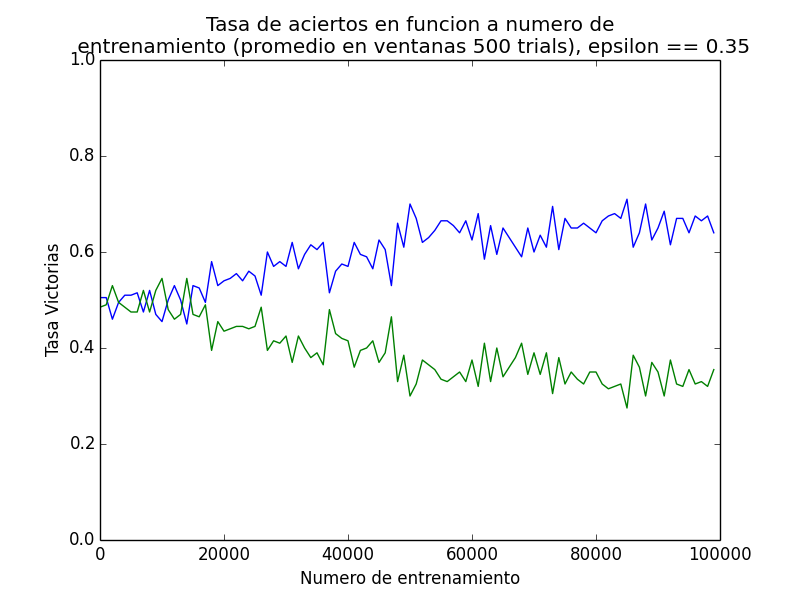
\includegraphics[scale=0.25]{q_vs_random_epsilon_0_35.png}
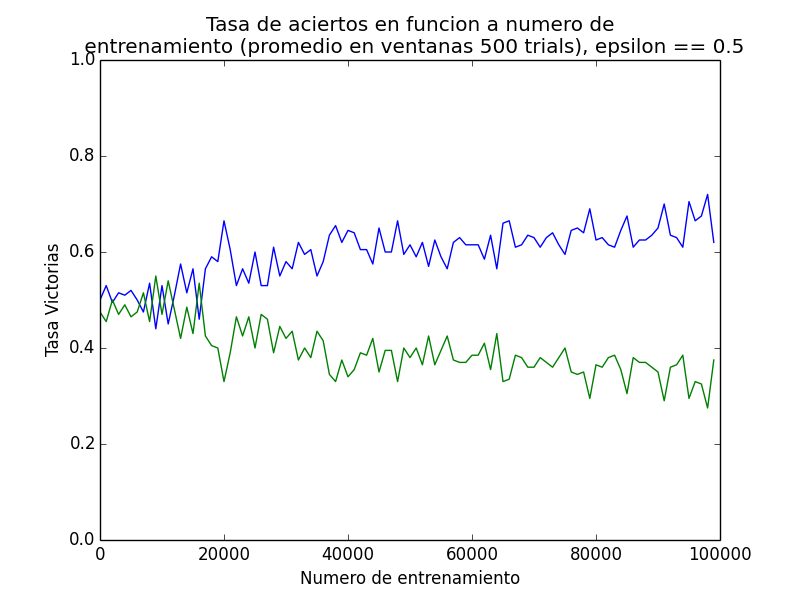
\includegraphics[scale=0.25]{q_vs_random_epsilon_0_5.png}
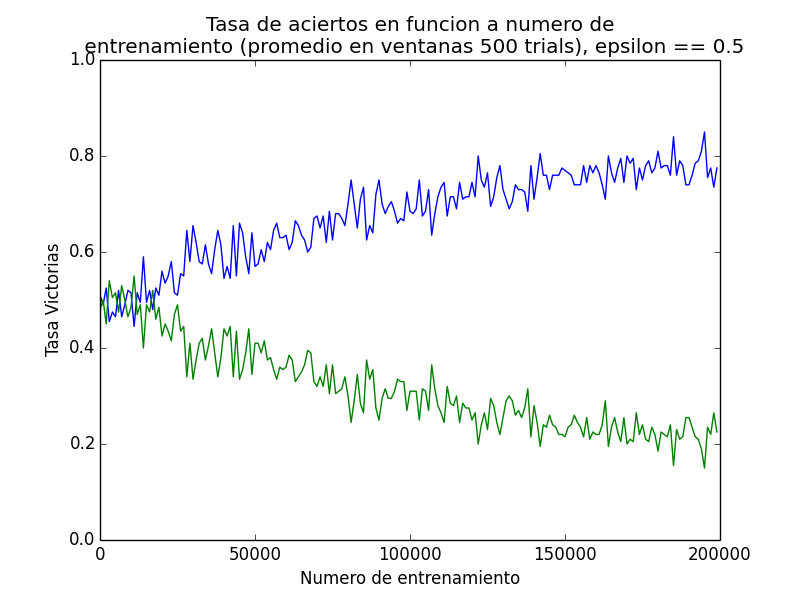
\includegraphics[scale=0.25]{q_vs_random_epsilon_0_5_200.png}
\\
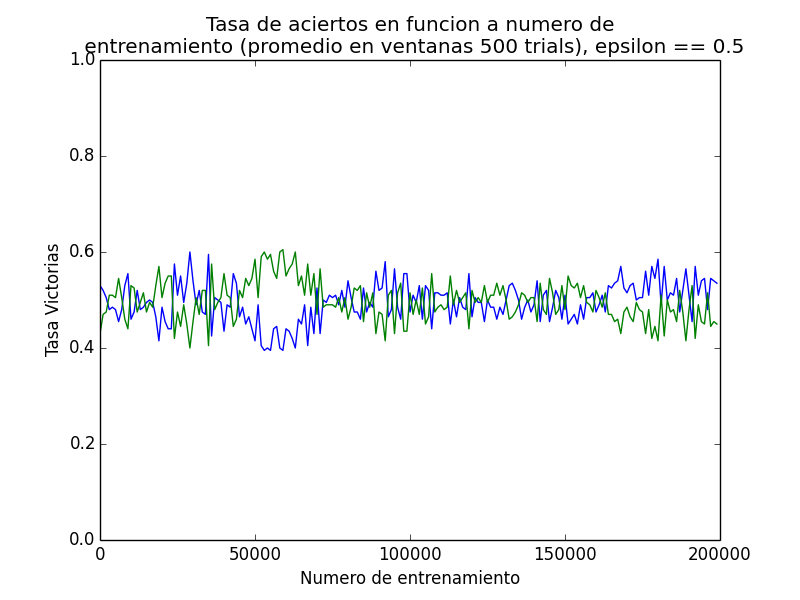
\includegraphics[scale=0.3]{q_vs_q_epsilon_0_5_200.png}
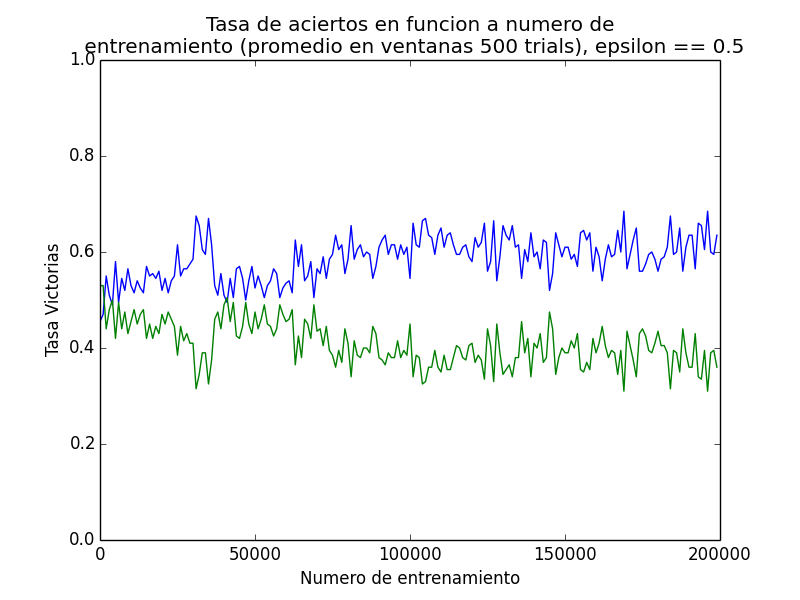
\includegraphics[scale=0.3]{q_vs_q_epsilion_0_5_200.png}

Los primeros tres gráficos muestran los resultados contra nuestro jugador \textit{random} mientras que los últimos dos representan dos corridas distintas de competencias entre los jugadores \textit{Q Learning}. En este segundo caso puede observarse un fenómeno particular, a saber, una diferencia notable en los \textit{rates} de victorias para dos corridas experimentales con idénticos parámetros. Si bien el aumento del épsilon aumenta la aleatoriedad y, por lo tanto, la posibilidad de diferencias, llama la atención cómo los \textit{rates} de victorias llegan a un régimen estable, fluctuando alrededor de un equilibrio. Este fenómeno refleja la relación existente entre los partidos jugados en el pasado (junto con sus resultados) y los partidos que nuestro jugador todavía no jugó. Si bien es difícil establecer con precisión cómo esa relación influye en concreto en favor de uno u otro resultado en el futuro, sí sabemos que una mayor cantidad de victorias previas configura un mapa cargado con más cantidad de indicaciones hacia 'casilleros' representando juegos victoriosos. Esto podría explicar las tendencias observadas previamente: en la disputa entre dos jugadores \textit{Q Learning} uno tome cierta ventaja sobre el otro, como un fenómeno del azar que toma peso en desiciones posteriores del algoritmo de aprendizaje.

\subsection{Variaciones sobre Alpha}
El hiperparámetro \textit{alpha} o \textit{learning rate} establece con qué rapidez una información 'nueva' reemplazará a la información previa. Representa el impacto que una experiencia contraria a aprendizajes anteriores puede generar. Mientras que un \textit{learning rate} igual a 0 indica que nuestro jugador no aprende nada, un \textit{learning rate} igual a 1 indica que sólo tomamos en consideración la última experiencia realizada en cuanto al valor de una jugada en un determinado tablero. Las experiencias previas fueron realizadas con un \textit{learning rate} con valor 0.8. A continuación estudiamos los efectos de modificar este hiperparámetro asignándole valores menores.

En primer lugar, observamos el resultado de entrenar nuestro jugador \textit{Q Learning} con parámetro \textit{alpha} igual a 0.2. Un valor bajo de \textit{alpha} retrasa las tendencia que se expresa con el aprendizaje. El algoritmo aprende más lento, entonces lo que aprende tarda más en manifestarse. Si observamos el \textit{ratio} de victorias luego de cien mil partidas jugadas observamos que los valores del jugador \textit{Q Learning} y del jugador \textit{random} están mucho más cercanos entre sí que si observamos los \textit{ratios} de las primeras figuras en la sección 3.1. Incluso al ver el resultado luego de doscientas mil partidas vemos que si bien ya se manifiesta una tendencia cercana al 80\% de victorias para el \textit{Q Learning}, aún no alcanza este valor, lo que sí sucede con mayor claridad en los ejemplos de la sección 3.1
\\
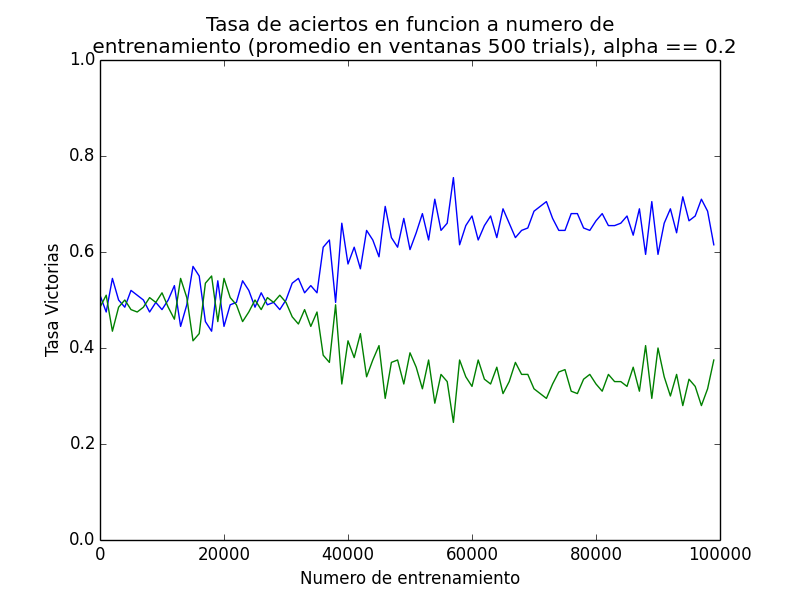
\includegraphics[scale=0.3]{q_vs_random_alpha_0_2.png}
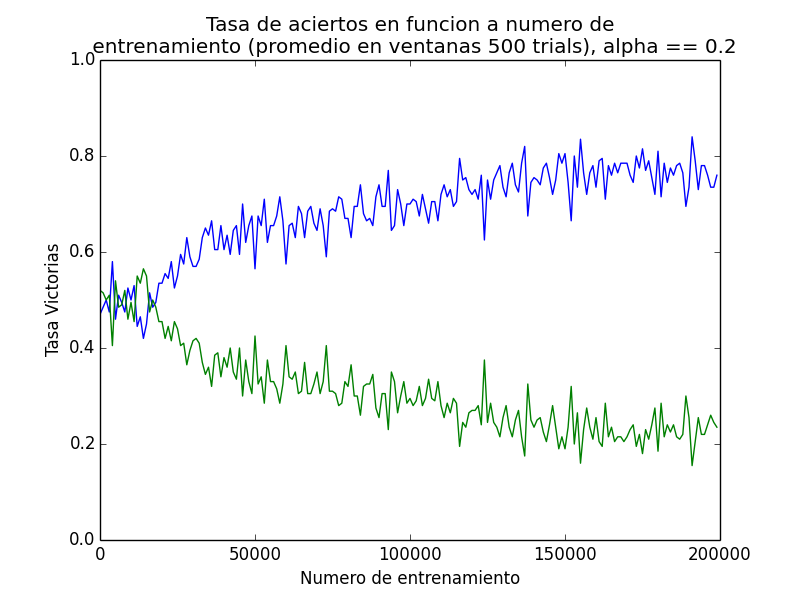
\includegraphics[scale=0.3]{q_vs_random_alpha_0_2_200.png}
\\
Por otro lado, para el mismo valor de \textit{alpha}, también puede observarse como se retrasa la tendencia que podía verse al enfrentar a dos jugadores \textit{Q Learning} entre sí: los \textit{ratios} de ambos jugadores son más cercanos y menos definidos como tendencia.
\\
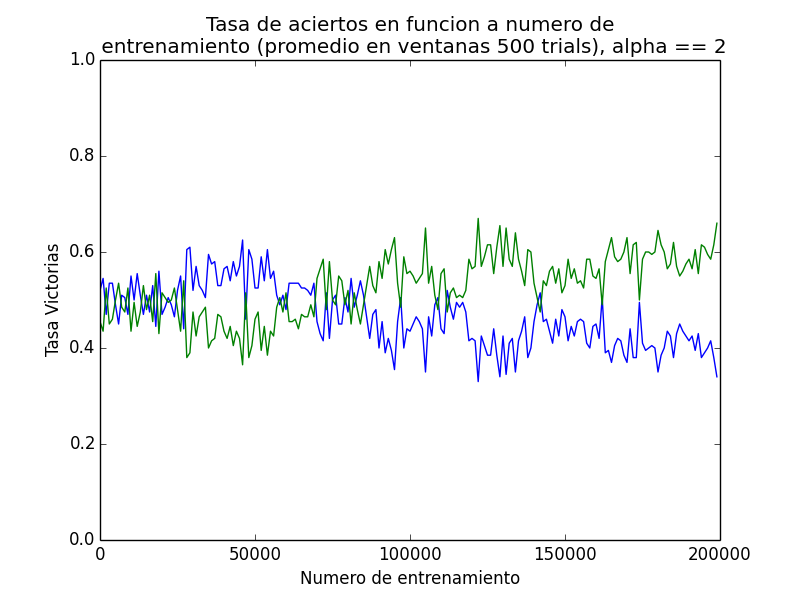
\includegraphics[scale=0.3]{q_vs_q_alpha_2_200.png}
\\
Por último, para los \textit{alphas} grandes (iguales a 1), un aprendizaje en una coordenada cercana a donde ya habíamos aprendido algo sobreescribe el resto de los aprendizajes. En consecuencia, estamos aprendiendo todo nuevamente, una y otra vez. La naturaleza del juego, además, puede generar tableros en los que la victoria de uno u otro jugador pueda depender de una sóla jugada de cada uno. Es decir que en el espacio de estados una situación victoriosa pueda darse `al lado' de una situación de derrota. Esto puede servir como ejemplo de lo que, según entendemos, no logra captar un aprendizaje con un parámetro alpha igual a 1. En consecuencia, obtenemos una situación curiosa en la que un jugador \textit{Q Learning} no logra superar a un jugador \textit{random}.\footnote{Vale aclarar que este experimento fue ejecutado cinco veces, todas con resultados similares.}
\\
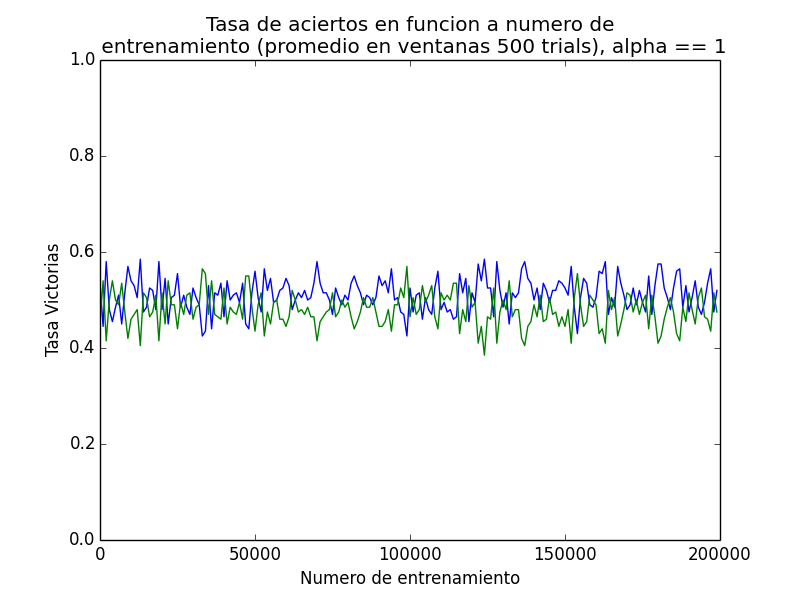
\includegraphics[scale=0.3]{q_vs_random_alpha_1_200_v2.png}
\\

\subsection{Variaciones sobre Gamma}

El parametro \textit{gamma} representa el \textit{discount factor}. Cuanto más bajo sea este parámetro, menos se esparcirá una recompensa positiva o negativa hacia los cuadrantes cercanos y, por lo tanto, menor será la influencia que tenga sobre estos. Si el discount factor es, por ejemplo, 0, el algoritmo de aprendizaje sólo será capaz de reconocer que se encuentra cerca de la victoria cuando esté a una jugada de distancia. Si por el contrario, el discount factor es 1, cada victoria se propagará infinitamente hacia todos los posibles casilleros, lo cual no permitiría distinguir entre un tablero en el que se puede ganar en una jugada de uno en el que se puede ganar en 20. A continuación observamos los resultados obtenidos luego de entrenar a nuestro jugador \textit{Q Learning} contra un jugador \textit{random} durante doscientas mil partidas con tres valores distintos de gamma: 0, 0.4 y 1
\\
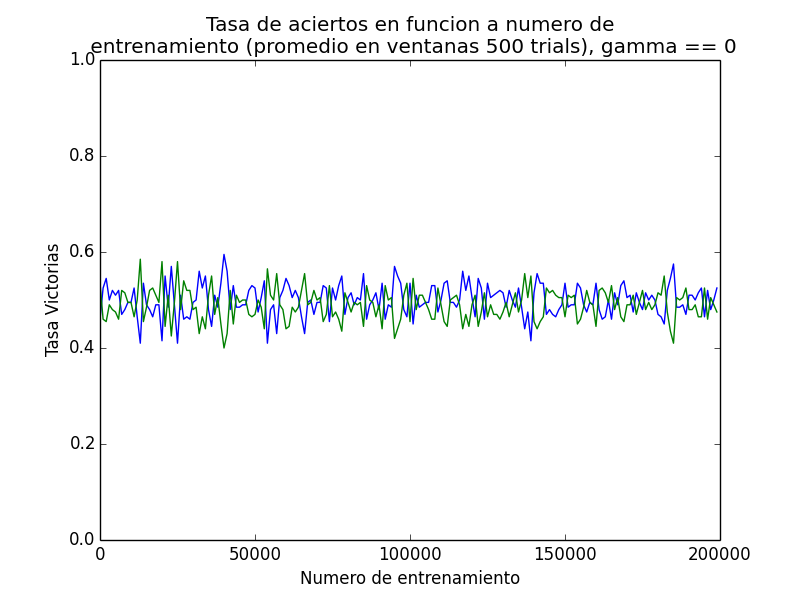
\includegraphics[scale=0.25]{q_vs_random_gamma_0_200.png}
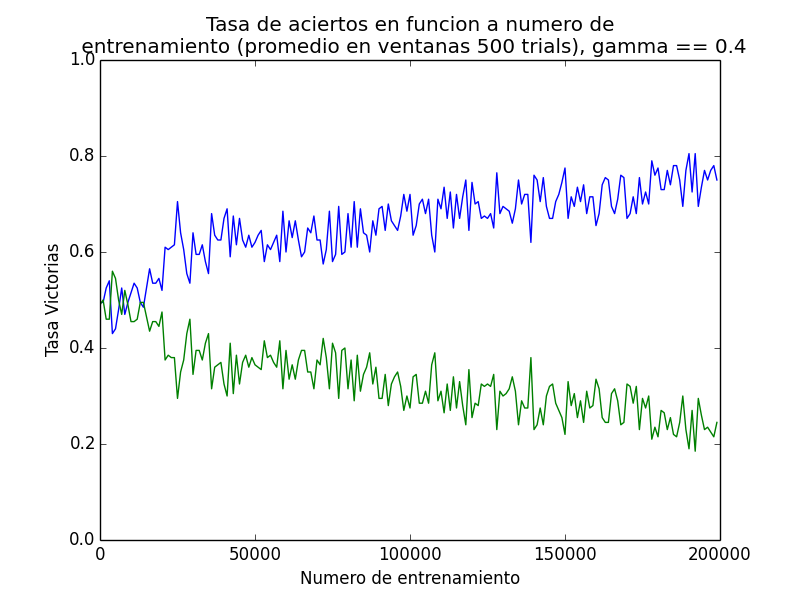
\includegraphics[scale=0.25]{q_vs_random_gamma_0_4_200.png}
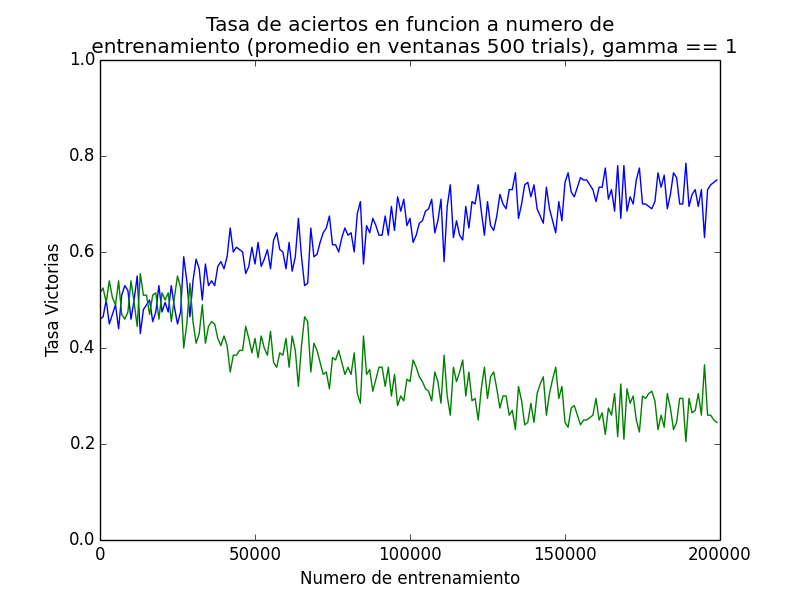
\includegraphics[scale=0.25]{q_vs_random_gamma_1_200.png}
\\

Los valores ideales de gamma, como esperabamos ver, son aquellos intermedios entre 0 y 1. Sin embargo, existe una diferencia sustancial entre valores de \textit{gamma} cercanos a 0 donde el aprendizaje no impacta, prácticamente, en las decisiones del jugador y valores cercanos a uno, donde si bien, los resultados no son los ideales, puede observarse claramente la tendencia a dominar en el juego por sobre el jugador \textit{random}.

\section{Conclusion}

Pudimos ver que a través del algoritmo de Q Learning, a pesar de ser relativamente simple y no estar diseñado específicamente para este juego -de hecho sin conocer sus reglas sino únicamente el resultado final y el espacio de estados posibles-, se puede obtener un desempeño considerable. Se alcanzaron tasas de ganancia de 0.82 de un jugador entrenado con Q Learning respecto a uno que jugaba al azar. Incluso al jugar un ser humano inexperto en el Cuatro en Línea (como los autores de este trabajo) contra un Q Learning suficientemente entrenado, difícilmente puede llegar a ganar el ser humano.

Uno de los resultados que nos sorprendio fue la aparente existencia de una estrategia ganadora para el jugador que arranca el juego.

Dado que es un juego finito y a un jugador lo unico que le importa es ganar, no cuanto tiempo le tome, conjeturamos que lo optimo es que el factor de descuento utilizado al calcular Q sea 1. En general se usa un factor de descuento menor a 1 en juegos que no son finitos para forzar a que el agente tome una desicion que lleve lo suficientemente rapido hacia una victoria.

\end{document}